\section{Python Loops}
\begin{figure}[ht]
	\centerline{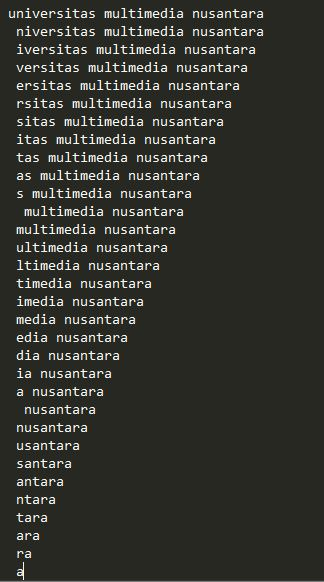
\includegraphics[width=0.25\textwidth]{gambar/perulangan}}
	\caption{Perulangan}
	\label{perulangan}
\end{figure}
Python dikenal sebagai bahasa pemograman interpreter, karena Python dieksekusi dengan sebuah interpreter. Satu hal yang telah kita ketahui bahwa bahasa pemograman Python adalah bahasa pemograman yang mudah dibaca dan terstruktur. Python sangat mementingkan indentasi, sehingga kita perlu melakukan indentasi secara konsisten. Indentasi tersebut dipermudah dengan penggunaan tombol Tab dan dimulai dari kolom pertama untuk setiap blok baru\cite{santoso2009bahasa}.
Python memiliki kelebihan lain yang sangat penting dibanding bahasa pemrograman yang terdahulu:
\begin{itemize}
\item Python merupakan open-source software, yang artinya ia dapat diperoleh secara gratis. Bahkan python sudah otomatis terinstall di Linux.
\item Python tersedia pada semua operating systems (OS) terkenal seperti Linux, Unix, Windows, dan MacOS. Suatu script python yang ditulis pada OS tertentu, dapat dijalankan di OS lain tapa ada modifikasi sedikitpun.
\item Python lebih mudah dipelajari sekaligus lebih mudah "‘dibaca"’ dibandingkan dengan bahasa pemrograman lainnya.
\item Python dan program ekstensinya mudah diinstall.
\end{itemize}
Python berdiri di atas landasan pondasi Java and C++. Hal-hal seperti classes, methods, inheritance, yang kerapkali diimplementasikan pada bahasa yang bersifat object-oriented, juga dapat diimplementasikan di python.\cite{suparno2013komputasi}

Secara umum, perulangan adalah blok kode yang dieksekusi berulang kali. Semua bahasa pemrograman menyediakan berbagai model struktur perulangan, seperti contohnya pada PHP ada while, for, dan foreach. Python juga menyediakan berbagai model tipe untuk menghandel perulangan. \par

Perintah perulangan di gunakan untuk mengulang pengeksekusian statemen-statemen hingga
berkali-kali sesuai dengan iterasi yang diinginkan. Dalam python, perintah untuk perulangan (loop)
adalah while dan for.

Secara umum, pernyataan pada bahasa pemrograman akan dieksekusi secara berurutan. Pernyataan pertama dalam sebuah fungsi dijalankan pertama, diikuti oleh yang kedua, dan seterusnya. Tetapi akan ada situasi dimana Anda harus menulis banyak kode, dimana kode tersebut sangat banyak. Jika dilakukan secara manual maka Anda hanya akan membuang-buang tenaga dengan menulis beratus-ratus bahkan beribu-ribu kode. Untuk itu Anda perlu menggunakan pengulangan di dalam bahasa pemrograman Python. \par

Di dalam bahasa pemrograman Python pengulangan dibagi menjadi 3 bagian, yaitu : 
\begin{itemize}
\item
While Loop 
\item
For Loop 
\item
Nested Loop 
\end{itemize} 
\vspace{\baselineskip}
\vspace{\baselineskip}
\vspace{12pt}


\subsection{While Loop}
Pengulangan While Loop di dalam bahasa pemrograman Python dieksesusi statement berkali-kali selama kondisi bernilai benar atau True. \par
\vspace{\baselineskip}
\vspace{\baselineskip}
Dibawah ini adalah contoh penggunaan pengulangan While Loop. \par
\vspace{\baselineskip}
\vspace{12pt}
Contoh penggunaan While Loop \par
\vspace{\baselineskip}
\vspace{\baselineskip}
\begin{verbatim}
count = 0 \par
while (count < 9): \par
 \$  \$  \$  \$ print ('The count is:', count) \par
 \$  \$  \$  \$ count = count + 1 \par
print ("Good bye!") \par
\end{verbatim}
\vspace{\baselineskip}
\vspace{\baselineskip}
\vspace{\baselineskip}
\vspace{12pt}

\subsection{For Loop}
Perulangan for disebut juga counted loop \(perulangan yang terhitung\)
Pengulangan for digunakan untuk pengulangan dengan muatan yang banyak\cite{van2007python}.
keistimewaan perulanga pada for adalah , perulangan dapat di hentikan pada saat kondisi tertentu. pada python, statemen for bekerja mengulang berbagai macam tipe data sekuensial seperti pada list, string dan tuple
Contohnya Seperti :
\begin{verbatim}
for a in range(0, 10):
	print a
\end{verbatim}
Hasil Outputnya :
\begin{verbatim}
python for.py
0
1
2
3
4
5
6
7
8
9
\end{verbatim}

Pengulangan For pada Python memiliki kemampuan untuk mengulangi item dari urutan apapun, seperti \$  \$list atau string. \par
\vspace{\baselineskip}
\vspace{\baselineskip}
Dibawah ini adalah contoh penggunaan pengulangan While Loop. \par
\vspace{\baselineskip}
\vspace{12pt}
Contoh pengulangan for sederhana \par
\vspace{\baselineskip}
angka = [1,2,3,4,5] \par
\vspace{\baselineskip}
for x in angka: \par
\vspace{\baselineskip}
 \$  \$  \$  \$ print(x) \par
\vspace{\baselineskip}
\vspace{\baselineskip}
Contoh pengulangan for \par
\vspace{\baselineskip}
buah = ["nanas", "apel", "jeruk"] \par
\vspace{\baselineskip}
for makanan in buah: \par
\vspace{\baselineskip}
 \$  \$  \$  \$ print(\"Saya suka makan\", makanan) \par
\vspace{\baselineskip}
\vspace{\baselineskip}
\vspace{12pt}

Looping artinya adalah pengulangan. Misalnya anda mendapat tugas untuk menghitung akar bilangan-bilangan dari 1 sampai 10. Ada 2 cara untuk menyelesaikan tugas tersebut, pertama, salinlah source-code berikut pada python editor lalu diberi nama looping01.py
\begin{enumerate}
\item from numpy import sqrt \# hanya function sqrt yang dipanggil
\item print sqrt(1)
\item print sqrt(2)
\item print sqrt(3)
\item print sqrt(4)
\item print sqrt(5)
\item print sqrt(6)
\item print sqrt(7)
\item print sqrt(8)
\item print sqrt(9)
\item print sqrt(10)
\end{enumerate}
Jalankan source-code di atas dengan menekan tombol F5, maka akan muncul hasil sebagai berikut :
\begin{enumerate}
\item 0
\item 41421356237
\item 73205080757
\item 0
\item 2360679775
\item 44948974278
\item 64575131106
\item 82842712475
\item 0
\item 16227766017
\end{enumerate}
Cara kedua dengan teknik looping, yaitu :
from numpy import sqrt
for i in range(1,10+1):
print sqrt(i)
Simpanlah source-code ini dengan nama looping02.py, lalu jalankan dengan F5, akan nampak
hasil yang sama yaitu
\begin{enumerate}
\item 0
\item 41421356237
\item 73205080757
\item 0
\item 2360679775
\item 44948974278
\item 64575131106
\item 82842712475
\item 0
\item 16227766017
\end{enumerate}

Mari sejenak kita bandingkan antara looping01.py dan looping02.py. Kedua source-code itu memiliki tujuan yang sama yaitu menghitung akar bilangan dari 1 sampai 10. Perbedaannya, looping01.py berisi 11 baris statemen, sedangkan looping02.py hanya 3 baris statemen. Coba cek
ukuran file-nya! Ukuran file looping01.py (di laptop saya) adalah 179 byte, sementara ukuran looping02.py adalah 72 byte. Dengan demikian dapat disimpulkan bahwa looping02.py lebih efisien dibanding looping01.py.\cite{suparno2013komputasi}

\subsection{Nested Loop}
Nested Loop (Perulangan Bertingkat) adalah semua tipe perulangan yang dapat dipakai di dalam perulangan yang lain. Jadi Perulangan for bisa dipakai di dalam for yang lain, perulangan for bisa berada didalam perulangan while, perulangan while bisa dipakai di dalam perulangan while yang lain, dan perulangan while bisa di dalam perulangan for. \par
\vspace{12pt}
Bahasa pemrograman Python memungkinkan penggunaan satu lingkaran di dalam loop lain. Bagian berikut menunjukkan beberapa contoh untuk menggambarkan konsep tersebut. \$  \$\vspace{\baselineskip}
\vspace{\baselineskip}
Dibawah ini adalah contoh penggunaan Nested Loop. \par

Contoh penggunaan Nested Loop : \par
\vspace{\baselineskip}
\vspace{\baselineskip}
i = 2 \par
\vspace{\baselineskip}
while(i < 100): \par
\vspace{\baselineskip}
 \$  \$  \$  \$ j = 2 \par
\vspace{\baselineskip}
 \$  \$  \$  \$ while(j <= (i/j)): \par
\vspace{\baselineskip}
 \$  \$  \$  \$  \$  \$  \$  \$ if not(i \$  \%  \$j): break \par
\vspace{\baselineskip}
 \$  \$  \$  \$  \$  \$  \$  \$ j = j + 1 \par
\vspace{\baselineskip}
 \$  \$  \$  \$ if (j > i/j) : print i, " is prime" \par
\vspace{\baselineskip}
 \$  \$  \$  \$ i = i + 1 \par
\vspace{\baselineskip}
\vspace{\baselineskip}
print "Good bye!" \par
\vspace{12pt}
\vspace{12pt}
Perhatikan contoh berikut ini:\vspace{\baselineskip}
\vspace{\baselineskip}
 \par
\vspace{12pt}
print ("1") \par
print ("2") \par
print ("3") \par
print ("4") \par
print ("5") \par
print ("6") \par
print ("7") \par
print ("8") \par
print ("9") \par
print ("10") \par
\vspace{12pt}
\vspace{\baselineskip}

Contoh program diatas adalah program untuk menampilkan angka 1 sampai dengan 10 tanpa perulangan. Tanpa menggunakan perulangan, programmer harus menuliskan semua statement diatas sehingga source code menjadi lebih banyak dan tidak efisien. Bayangkan kalau programmer disuruh menampilkan angka 1 sampai dengan 1000000 tanpa menggunakan perulangan\vspace{\baselineskip}
\vspace{\baselineskip}

Dengan menggunakan perulangan, source code lebih pendek dan efisien. Perhatikan contoh program untuk mencetak angka 1 sampai dengan 10 dengan menggunakan konsep perulangan di bawah ini.\vspace{\baselineskip}
\vspace{\baselineskip}
 \par
\vspace{12pt}

begin{verbatim}
i = 1 \par
while(i < 11): \par
~~~ print(i) \par
~~~ i = i+1 \par
end{verbatim}
\vspace{\baselineskip}

Bandingkan kedua program diatas, Mana yang lebih efisien? Mana yang lebih simple?\vspace{\baselineskip}
\vspace{\baselineskip}

Ada 3 macam bentuk perulangan pada Python, yaitu: \par
FOR Loop \par
WHILE Loop \par
dan Loop bersarang (Nested Loop) \par
\vspace{\baselineskip}

Selain membahas 3 bentuk perulangan diatas, tutorial ini juga membahas control perulangan, meliputi: \par
Break Statement \par
Continue Statement \par
dan Pass Statement \par
\vspace{\baselineskip}
\vspace{12pt}

\subsubsection{Contoh Penggunaan Nested Loop}
Format nested loop \(for di dalam for\)
\begin{verbatim}
For iterasi_var_1 in urutan_1:
	Statements_untuk_perulangan_for_yang_di_luar
...
For iterasi_var_1 in urutan_2:
	Statements_untuk_perulangan_for_yang_di_dalam
...
Statements_untuk_perulangan_for_yang_di_luar
...
\end{verbatim}

Format nested loop \(while di dalam while\)
\begin{verbatim}
While expressions:
	Statements_untuk_perulangan_while_yang_di_dalam
...
Statements_untuk_perulangan_whle_yang_di_luar
...
\end{verbatim}

Contoh :
\begin{verbatim}
X = int(input(“Masukkan jumlah bariss: “))
For i in range (x) :
	For j in range(i+1):
		Print(“*”, end=””)
	Print()
\end{verbatim}
Saat di Run Module maka :
Masukkan jumlah bariss: 5 \(inputkan 5\)
*
**
***
****
***** 
Muncul 5 baris isi bintang

\subsubsection{Nested Loop for Nested Data}
Disini kita memiliki list data dari murid-murid. Jadi, setiap murid memiliki nama yang dipasangkan dengan list subyek(mata pelajaran) yang mereka ambil. Dan akan mencetak setiap nama murid, dan jumlah dari subyek (mata pelajaran) yang mereka ambil
\begin{verbatim}
students = [
    ("John", ["TIK", "IPS"]),
    ("Vusi", ["Matematika", "TIK", "IPA"]),
    ("Jess", ["TIK", "Bahasa Indonesia", "Ekonomi", "Pendidikan Agama Islam"]),
    ("Sarah", ["Biologi", "Matematika", "Ekonomi", "Kimia"]),
    ("Zuki", ["Sosiologi", "Ekonomi", "Biologi", "Matematika", "Bahasa Inggris"])]

for (name, subjects) in students:
    print(name, "takes", len(subjects), "courses")
\end{verbatim}
Lalu, setelah dijalankan (run) maka akan tampil seperti ini:
John takes 2 courses
Vusi takes 3 courses
Jess takes 4 courses
Sarah takes 4 courses
Zuki takes 5 course

\subsection{FOR Loop}
FOR Loop digunakan untuk melakukan perulangan atau iterasi sampai batas atau range yang telah ditentukan.\vspace{\baselineskip}
\vspace{\baselineskip}
Dibawah ini adalah sintak dasar FOR Loop di Python.\vspace{\baselineskip}
\vspace{\baselineskip}
 \par
for iterating \$  \_  \$var in range: \par
~~ statements(s) \par
\vspace{\baselineskip}
Contoh Program\vspace{\baselineskip}
\vspace{\baselineskip}
Perhatikan contoh program For Loop pada Python:\vspace{\baselineskip}
\vspace{\baselineskip}
Contoh 1\vspace{\baselineskip}
\vspace{\baselineskip}
 \par
 \begin{equation}
 Program mencetak angka 1 s/d 10 
 \end{equation}
\vspace{12pt}
\begin{verbatim}
i = 10 \par
for i in range(10): \par
~~ print(i+1) \par
~~ i = i+1 \par
\end{verbatim}
\vspace{\baselineskip}
Fungsi \$  \$range() \$  \$biasanya digunakan sebagai counter pada perulangan bentuk For. range(10) artinya menampikan perulangan sebanyak 10 elemen.\vspace{\baselineskip}
\vspace{\baselineskip}
Apabila program diatas Anda jalankan, maka akan menampilkan angka 1 sampai dengan 10 seperti output di bawah ini:\vspace{\baselineskip}
\vspace{\baselineskip}
 \par
1 \par
2 \par
3 \par
4 \par
5 \par
6 \par
7 \par
8 \par
9 \par
10 \par
\vspace{\baselineskip}
Contoh 2\vspace{\baselineskip}
\vspace{\baselineskip}
 \par
 Program mencetak angka -1 s/d 8 \par
\vspace{12pt}
begin{verbatim}
i = 10 \par
for i in range(-10, 10, 2):  \$  \#  \$ range(range awal, range akhir, selisih) \par
~~ print(i) \par
end{verbatim}
\vspace{12pt}
\vspace{\baselineskip}
Perhatikan pada range(-10, 10, 2) artinya perulangan akan dimulai dari batas awal -10 sampai dengan batas akhir 10 dengan selisih 2.\vspace{\baselineskip}
\vspace{\baselineskip}
Apabila program diatas Anda jalankan, maka akan menampilkan output berikut ini:\vspace{\baselineskip}
\vspace{\baselineskip}
 \par
-10 \par
-8 \par
-6 \par
-4 \par
-2 \par
0 \par
2 \par
4 \par
6 \par
8 \par
\vspace{\baselineskip}
Contoh 3\vspace{\baselineskip}
\vspace{\baselineskip}
 \par
Program menampilkan huruf Belajar Python \par
for~huruf~in 'Belajar Python':    \par
~~ print (huruf) \par
\vspace{\baselineskip}
Apabila program diatas Anda jalankan, maka akan menghasilkan output berikut ini:\vspace{\baselineskip}
\vspace{\baselineskip}
 \par
B \par
e \par
l \par
a \par
j \par
a \par
r \par
  \par
P \par
y \par
t \par
h \par
o \par
n \par
\vspace{12pt}
Contoh 4\vspace{\baselineskip}
\vspace{\baselineskip}
Program berikut akan menampilkan perulangan dari list atau tupple.\vspace{\baselineskip}
\vspace{\baselineskip}
 \par
Program menampilkan huruf Belajar Python \par
\vspace{12pt}
begin{verbatim}
makanan = ['Pizza', 'Nasi Bebek',~ 'Rujak Buah'] \par
for makan in makanan: \par
~~ print (\"Makanan Favorit :\", makan) \par
end{verbatim}
\vspace{12pt}
Apabila program diatas Anda jalankan, maka akan menghasilkan output berikut ini:\vspace{\baselineskip}
\vspace{\baselineskip}
 \par
Makanan Favorit : Pizza \par
Makanan Favorit : Nasi Bebek \par
Makanan Favorit : Rujak Buah \par
\vspace{12pt}
\vspace{\baselineskip}
\vspace{12pt}
\subsection{While Loop}
While Loop akan menjalankan statemet selama kondisi terpenuhi (atau bernilai true).\vspace{\baselineskip}
\vspace{\baselineskip}
Di bawah ini adalah sintak dasar dari While Loop pada Python\vspace{\baselineskip}
\vspace{\baselineskip}
Contoh Program\vspace{\baselineskip}
\vspace{\baselineskip}
Coba Anda ketik program di bawah ini:\vspace{\baselineskip}
\vspace{\baselineskip}
 \par
Program mencetak angka 1 s/d 10 \par
\vspace{12pt}
begin{verbatim}
i = 1 \par
while(i < 11): \par
 print(i) \par
 i = i+1 \par
 end{verbatim}
\vspace{\baselineskip}

Apabila program diatas Anda jalankan, maka akan menghasilkan output seperti di bawah ini:\vspace{\baselineskip}
\vspace{\baselineskip}
 \par
1 \par
2 \par
3 \par
4 \par
5 \par
6 \par
7 \par
8 \par
9 \par
10 \par
\vspace{12pt}
\vspace{\baselineskip}
\vspace{12pt}
\subsection{Infinite Loop}
\vspace{\baselineskip}
Infinite Loop adalah kondisi perulangan, dimana statement akan dijalankan terus menerus tanpa berhenti. Akan berhenti kalau Anda menekan tombol CTRL+C.\vspace{\baselineskip}
\vspace{\baselineskip}
Di bawah ini contoh program Infinite Loop\vspace{\baselineskip}
\vspace{\baselineskip}
 \par
program menampilkan tulisan Python tanpa henti \par
\vspace{12pt}
flag = 1 \par
\vspace{12pt}
while (flag): print ("Python") \par
print ("Good bye!") \par
\vspace{12pt}
\vspace{\baselineskip}
\vspace{12pt}
\subsection{Nested Loop}
\vspace{\baselineskip}
Nested Loop secara sederhana adalah perulangan di dalam perulangan.\vspace{\baselineskip}
\vspace{\baselineskip}
Di bawah ini adalah sintak dasar Nested Loop pada Python:\vspace{\baselineskip}
\vspace{\baselineskip}
 \par
for iterating \$  \_  \$var in sequence: \par
~~ for iterating \$  \_  \$var in sequence: \par
~~~~~ statements(s) \par
~~ statements(s) \par
\vspace{\baselineskip}
atau yang menggunakan while loop\vspace{\baselineskip}
\vspace{\baselineskip}
 \par
while expression: \par
~~ while expression: \par
~~~~~ statement(s) \par
~~ statement(s) \par
\vspace{\baselineskip}
Contoh Program\vspace{\baselineskip}
\vspace{\baselineskip}
Di bawah ini adalah contoh program implementasi Nested Loop untuk mencetak bilangan prima dari 2 sampai 30.\vspace{\baselineskip}
\vspace{\baselineskip}
 \par
Program menampilkan bilangan prima dari 2 s/d 30 \par
\vspace{12pt}
\begin{verbatim}
i = 2 \par
while(i < 30): \par
~~ j = 2 \par
~~ while(j <= (i/j)): \par
~~~~~ if not(i \$  \%  \$j): break \par
~~~~~ j = j + 1 \par
~~ if (j > i/j) : print (i, \" adalah bilangan prima\") \par
~~ i = i + 1 \par
\end{verbatim}
\vspace{12pt}
print (\"Good bye!\") \par
\vspace{12pt}
\vspace{\baselineskip}
Apabila program diatas Anda jalankan, maka akan menampilkan output seperti di bawah ini.\vspace{\baselineskip}
\vspace{\baselineskip}
 \par
2~ adalah bilangan prima \par
3~ adalah bilangan prima \par
5~ adalah bilangan prima \par
7~ adalah bilangan prima \par
11~ adalah bilangan prima \par
13~ adalah bilangan prima \par
17~ adalah bilangan prima \par
19~ adalah bilangan prima \par
23~ adalah bilangan prima \par
29~ adalah bilangan prima \par
\vspace{12pt}
Pengulangan adalah salah satu hal penting yang ada di bahasa pemrograman. Pengulangan digunakan misalnya untuk meng-update \$  \$nama \$  \$file \$  \$yang cukup banyak jumlahnya, atau mengakses piksel satu persatu pada gambar. \par
Python memiliki tiga jenis pengulangan yang wajib Anda cermati untuk membuat sebuah aplikasi dengan Python. Pengulangan yang pertama adalah \$  \$while. Dengan menggunakan \$  \$while, Anda dapat membuat kondisi tertentu untuk menghentikan \$  \$while. Biasanya \$  \$while \$  \$digunakan untuk melakukan \$  \$loopingyang tidak pasti. Coba lihat contoh berikut (Anda dapat menulisnya dalam sebuah \$  \$file, kemudian eksekusi \$  \$file \$  \$tersebut di konsol): \par
begin{verbatim}
i = 0 \par
while True: \par
~~~ if i < 10: \par
~~~~~~~ print "Saat ini i bernilai: ", i \par
~~~~~~~ i = i + 1 \par
~~~ elif i >= 10: \par
~~~~~~~ break \par
end{verbatim}
\vspace{12pt}
Pada potongan kode diatas, \$  \$while \$  \$akan terus berputar selama i masih kurang dari 10. Jika sudah lebih dari 10 maka \$  \$while \$  \$akan berhenti. Pengulangan \$  \$whilejuga biasa digunakan di aplikasi konsol, untuk menahan \$  \$user \$  \$mengisikan semua input yang diperlukan dan baru akan berhenti setelah semua input dan proses interaksi berakhir. Jika kode diatas kita jalankan, maka \$  \$output-nya akan seperti ini: \par
\vspace{12pt}
Saat~ini i bernilai:  0 \par
Saat~ini i bernilai:  1 \par
Saat~ini i bernilai:  2 \par
Saat~ini i bernilai:  3 \par
Saat~ini i bernilai:  4 \par
Saat~ini i bernilai:  5 \par
Saat~ini i bernilai:  6 \par
Saat~ini i bernilai:  7 \par
Saat~ini i bernilai:  8 \par
Saat~ini i bernilai:  9 \par
\vspace{12pt}
Sekarang kita coba gunakan \$  \$for. Pengulangan \$  \$for \$  \$biasa digunakan untuk pengulangan yang sudah jelas banyaknya. Misal, Anda ingin mengulang sebuah pengulangan sampai 10 kali atau mengeluarkan semua hasil \$  \$query \$  \$dari \$  \$databasedi halaman HTML. Berikut ini adalah contoh kode untuk pengulangan \$  \$for: \par
for i in range(0, 10): \par
~~~ print i \par
Jika dijalankan maka kode diatas akan mengeluarkan \$  \$output \$  \$seperti ini: \par
\vspace{12pt}
0 \par
1 \par
2 \par
3 \par
4 \par
5 \par
6 \par
7 \par
8 \par
9 \par
Tidak hanya mengiterasi deretan angka, pengulangan \$  \$for \$  \$pun dapat Anda gunakan untuk mengulang sesuatu yang \$  \$iterable \$  \$seperti \$  \$list, \$  \$tuple, \$  \$dictionary, dan \$  \$iterable object \$  \$lainnya. Berikut ini kita ambil contoh dengan mengulang sebuah \$  \$list \$  \$yang berisi karakter anime Dragonball Super: \par
\vspace{12pt}
dragonball \$  \_  \$super \$  \_  \$character = [\"Son Goku\", \"Vegeta\", \"Beerus\", \"Trunks\", \"Whiz\", \"Champa\"] \par
for character in dragonball \$  \_  \$super \$  \_  \$character: \par
~~~ print character \par
\vspace{12pt}
Jika kita jalankan potongan kode tadi, maka \$  \$output-nya akan seperti berikut: \par
\vspace{12pt}
\begin{itemize}
\item
Son Goku
\item
Vegeta
\item
Beerus
\item
Trunks
\item
Whiz
\item
Champa
\item
For Loop
\end{itemize}
Seperti pada bahasa pemrograman lainnya, for loop sudah menjadi standar namun berbeda-beda tata cara penulisan nya di setiap pemrograman. \par
\vspace{12pt}
Sekarang kita langsung buat contoh di Python. \$  \$ \par
\vspace{12pt}
\vspace{12pt}
Contoh iterasi pada String  \par
\vspace{12pt}
\begin{verbatim}
for~n in 'Python':   \par
~~~ print 'Huruf :', n \par
\end{verbatim}
\vspace{12pt}
  \par
iterasi pada List biasa \par
\vspace{12pt}
mobil = ['sedan', 'truk', 'angkot']  \par
for p in mobil: \par
~~~ print 'Mobil :', mobil \par
\vspace{12pt}
\vspace{12pt}
iterasi pada list melalui index \par
for i in range(len(mobil)): \par
~~~ print 'Mobil :', mobil[i] \par
\vspace{12pt}
iterasi angka / range \par
\vspace{12pt}
for a in range(1,10): \par
~~~~ print "Angka :", a \par
~~~~ if(a == 5):  \$  \#  \$ditambah conditional \par
~~~~~~~~ print "Saya dapat angka : ",a \par
\vspace{12pt}
iterasi loop nested \par
for a in range(1,10): \par
~~~ for x in range(11,20): \par
~~~~~~~~b~=~a~* x      \par
~~~~~~~ print "Angka :", b \par
\vspace{12pt}
loop dgn break \par
for letter in 'Python': \par
~~ if letter == 'h': \par
~~~~~ break \par
~~ print 'Current Letter :', letter \par
\vspace{12pt}
print "Good job !!!" \par
\vspace{12pt}
\subsection{While Loop}
WHile dipakai untuk looping dimana iterasi akan dilakukan selama kondisi yang diberikan benar. While ini juga bisa di pakai untuk Infinite loop. \par
\vspace{12pt}
Contoh While \par
count = 0 \par
while count < 100: \par
 \$  \$  \$  \$  \$  \$print "Count ke : ", count \par
 \$  \$  \$  \$  \$  \$count = count + 1 \par
\vspace{12pt}
infinite loop \par
''' \par
Set loop ini untuk kondisi dimana suatu syarat tidak pernah TRUE \par
''' \par
\vspace{12pt}
setvar =1 \par
while setvar == 1 \par
 \$  \$  \$  \$ input = input \$  \_  \$raw("Masukan angka :") \par
 \$  \$  \$  \$ print "Angka anda : ", input \par
\vspace{12pt}
loop diatas akan berhenti jika anda stop manual misal dgn CTRL+C di terminal \par
''' \par
ELSE statement di while loop. di Python kita bisa set WHile loop lalu dikasih kondisi \par
''' \par
\begin{verbatim}
count = 0 \par
while count < 5: \par
 \$  \$  \$  \$  \$  \$print "count : ",count \par
 \$  \$  \$  \$  \$  \$count = count + 1 \par
else: \par
 \$  \$  \$  \$ print "Lihat yang masuk sini apa : ",count \par
 \end{verbatim}
\vspace{12pt}
while dgn break \par
angka~=~10~~~~~~    \par
while~angka~>~0:~~~~~~~~~~     \par
~~  \par
~~ print 'Angka :', angka \par
~~ angka = angka -1 \par
~~ if angka == 7: \par
~~~~~ break \par
\vspace{\baselineskip}
\vspace{12pt}
\vspace{12pt}

\subsection{Penggunaan loop dengan else statement}
Python mendukung untuk memiliki pernyataan lain yang terkait dengan pernyataan lingkaran
Jika else statement digunakan dengan for loop, pernyataan yang lain dijalankan saat loop telah habis mengulangi daftar.
Jika else statement digunakan dengan loop sementara, pernyataan yang lain dijalankan saat kondisinya menjadi salah.

\subsection{Middle-test loop}
Middle-test loop adalah sebuah perulangan yang akan mengeksekusi pada beberapa bagian body, kemudian akan melakukan pengujian exit berarti menguji dalam kondisi exit, lalu kemungkinan akan mengeksekusi beberapa bagian body lainnya. Disini dapat menggunakan while dan break secara bersama-sama. Terkadang kita membutuhkan looping dengan pengujian di tengah daripada pengujian di atas maupun di akhir.

\subsection{Penjelasan Penggunaan For Loop}
For loop secara tradisional digunakan saat Anda memiliki blok kode yang ingin Anda ulangi beberapa kali. Python untuk pernyataan iterates atas anggota urutan dalam urutan, mengeksekusi blok setiap waktu. Kontras untuk pernyataan dengan loop '' while '', digunakan bila suatu kondisi perlu diperiksa setiap iterasi, atau untuk mengulang blok kode selamanya.
